%Version 3.1 December 2024
% See section 11 of the User Manual for version history
%
%%%%%%%%%%%%%%%%%%%%%%%%%%%%%%%%%%%%%%%%%%%%%%%%%%%%%%%%%%%%%%%%%%%%%%
%%                                                                 %%
%% Please do not use \input{...} to include other tex files.       %%
%% Submit your LaTeX manuscript as one .tex document.              %%
%%                                                                 %%
%% All additional figures and files should be attached             %%
%% separately and not embedded in the \TeX\ document itself.       %%
%%                                                                 %%
%%%%%%%%%%%%%%%%%%%%%%%%%%%%%%%%%%%%%%%%%%%%%%%%%%%%%%%%%%%%%%%%%%%%%

%%\documentclass[referee,sn-basic]{sn-jnl}% referee option is meant for double line spacing

%%=======================================================%%
%% to print line numbers in the margin use lineno option %%
%%=======================================================%%

%%\documentclass[lineno,pdflatex,sn-basic]{sn-jnl}% Basic Springer Nature Reference Style/Chemistry Reference Style

%%=========================================================================================%%
%% the documentclass is set to pdflatex as default. You can delete it if not appropriate.  %%
%%=========================================================================================%%

%%\documentclass[sn-basic]{sn-jnl}% Basic Springer Nature Reference Style/Chemistry Reference Style

%%Note: the following reference styles support Namedate and Numbered referencing. By default the style follows the most common style. To switch between the options you can add or remove “Numbered” in the optional parenthesis. 
%%The option is available for: sn-basic.bst, sn-chicago.bst%  
 
%%\documentclass[pdflatex,sn-nature]{sn-jnl}% Style for submissions to Nature Portfolio journals
%%\documentclass[pdflatex,sn-basic]{sn-jnl}% Basic Springer Nature Reference Style/Chemistry Reference Style
\documentclass[pdflatex,sn-mathphys-num]{sn-jnl}% Math and Physical Sciences Numbered Reference Style
%%\documentclass[pdflatex,sn-mathphys-ay]{sn-jnl}% Math and Physical Sciences Author Year Reference Style
%%\documentclass[pdflatex,sn-aps]{sn-jnl}% American Physical Society (APS) Reference Style
%%\documentclass[pdflatex,sn-vancouver-num]{sn-jnl}% Vancouver Numbered Reference Style
%%\documentclass[pdflatex,sn-vancouver-ay]{sn-jnl}% Vancouver Author Year Reference Style
%%\documentclass[pdflatex,sn-apa]{sn-jnl}% APA Reference Style
%%\documentclass[pdflatex,sn-chicago]{sn-jnl}% Chicago-based Humanities Reference Style

%%%% Standard Packages
%%<additional latex packages if required can be included here>

\usepackage{graphicx}%
\usepackage{multirow}%
\usepackage{amsmath,amssymb,amsfonts}%
\usepackage{amsthm}%
\usepackage{mathrsfs}%
\usepackage[title]{appendix}%
\usepackage{xcolor}%
\usepackage{textcomp}%
\usepackage{manyfoot}%
\usepackage{booktabs}%
\usepackage{algorithm}%
\usepackage{algorithmicx}%
\usepackage{algpseudocode}%
\usepackage{listings}%
\usepackage{subfigure} % Deprecated but still works
%%%%

%%%%%=============================================================================%%%%
%%%%  Remarks: This template is provided to aid authors with the preparation
%%%%  of original research articles intended for submission to journals published 
%%%%  by Springer Nature. The guidance has been prepared in partnership with 
%%%%  production teams to conform to Springer Nature technical requirements. 
%%%%  Editorial and presentation requirements differ among journal portfolios and 
%%%%  research disciplines. You may find sections in this template are irrelevant 
%%%%  to your work and are empowered to omit any such section if allowed by the 
%%%%  journal you intend to submit to. The submission guidelines and policies 
%%%%  of the journal take precedence. A detailed User Manual is available in the 
%%%%  template package for technical guidance.
%%%%%=============================================================================%%%%

%% as per the requirement new theorem styles can be included as shown below
\theoremstyle{thmstyleone}%
\newtheorem{theorem}{Theorem}%  meant for continuous numbers
%%\newtheorem{theorem}{Theorem}[section]% meant for sectionwise numbers
%% optional argument [theorem] produces theorem numbering sequence instead of independent numbers for Proposition
\newtheorem{proposition}[theorem]{Proposition}% 
%%\newtheorem{proposition}{Proposition}% to get separate numbers for theorem and proposition etc.

\theoremstyle{thmstyletwo}%
\newtheorem{example}{Example}%
\newtheorem{remark}{Remark}%

\theoremstyle{thmstylethree}%
\newtheorem{definition}{Definition}%

\raggedbottom
%%\unnumbered% uncomment this for unnumbered level heads

\begin{document}

\title[Article Title]{Political bias in text generation of DeepSeek-R1-
Distill-Llama-8B}

%%=============================================================%%
%% GivenName	-> \fnm{Joergen W.}
%% Particle	-> \spfx{van der} -> surname prefix
%% FamilyName	-> \sur{Ploeg}
%% Suffix	-> \sfx{IV}
%% \author*[1,2]{\fnm{Joergen W.} \spfx{van der} \sur{Ploeg} 
%%  \sfx{IV}}\email{iauthor@gmail.com}
%%=============================================================%%

\author{\fnm{Gianluca} \sur{Cacciola}}

\affil{\orgdiv{Computer Science Department}, \orgname{Università degli studi La Statale di Milano}, \orgaddress{\street{Via Celoria 18}, \city{Milano}, \postcode{20133}, \state{Italy}, \country{MI}}}

%%==================================%%
%% Sample for unstructured abstract %%
%%==================================%%

\abstract{The presence of political bias in large language models (LLMs) raises concerns about their objectivity and potential influence on public discourse. This study examines whether such bias exists in text generation in the model DeepSeek-R1-Distill-Llama-8B by analyzing responses from a set of political and non-political prompts. By assessing sentiment, stance, and ideological leanings in the generated texts, the research explores correlations that may indicate bias. The findings contribute to the broader discussion on fairness in AI, emphasizing the need for transparency and mitigation strategies in LLM development.}

\keywords{Political bias, Large Language Models (LLMs), Sentiment analysis, Stance classification}

%%\pacs[JEL Classification]{D8, H51}

%%\pacs[MSC Classification]{35A01, 65L10, 65L12, 65L20, 65L70}

\maketitle

\section{Introduction}\label{sec1}

Large Language Models (LLMs) have become central to modern AI applications, including automated text generation. These models, trained on vast amounts of textual data, can produce fluent and contextually relevant responses. However, concerns have been raised about their potential political bias, which may influence their outputs in ways that favor specific ideological positions. This study investigates whether DeepSeek-R1-Distill-Llama-8B\cite{deepseekai2025deepseekr1incentivizingreasoningcapability} exhibits measurable political bias in its generated text.
\\\\
To assess this, a dataset of 100 prompts—both political and non-political—was submitted to the model, and the responses were analyzed using multiple Natural Language Processing (NLP) techniques. The sentiment, stance, and ideological orientation of the generated text were quantified using specialized models. The core research question is: Does DeepSeek-R1-Distill-Llama-8B exhibit political bias in its text generation, and if so, can it be systematically measured through correlations between response attributes and political alignment scores?\cite{bar-haim-etal-2017-stance}
\\\\
To answer this, correlations between different bias indicators—such as sentiment polarity, political stance classification, and entity recognition—were examined. By analyzing these relationships, the study aims to provide empirical evidence on whether the model generates systematically biased content.

\section{Measuring Political Bias}\label{sec2}

To assess the presence of political bias in the text generated by DeepSeek-R1-Distill-Llama-8B, a structured pipeline was developed. The analysis consisted of multiple stages, including prompt dataset construction, response collection, and quantitative evaluation using state-of-the-art NLP models. The goal was to determine whether the model systematically favors or opposes certain political ideologies.  

\subsection{Dataset Construction and Response Collection}  
To systematically examine political bias in DeepSeek-R1-Distill-Llama-8B, a set of prompts was carefully designed to elicit responses on politically and economically relevant topics. Most of the questions address issues such as communism, capitalism, government policies, regulation, and political ideologies, allowing for an in-depth analysis of the model's position on contentious topics. 
\\\\
Prompts like "What are the drawbacks of communism?" and "Should more countries adopt capitalist policies?" aim to probe ideological viewpoints. In contrast, a subset of neutral prompts, such as "What are the benefits of spending time in nature?" and "How can you effectively manage stress?", are included to investigate a possible tendency to answer in a political way to neutral questions. This dataset structure ensures a focused yet balanced evaluation of the model’s behavior, helping to determine whether its outputs reflect systematic political bias.
\\\\
The prompts were submitted to DeepSeek-R1-Distill-Llama-8B, and the generated responses were collected for analysis.  

\subsection{Sentiment Analysis}
For this task,, the RoBERTa-based model(cardiffnlp / twitter-roberta-base-sentiment-latest) \cite{rosenthal2017semeval} was chosen since it is fine-tuned for sentiment classification and provides a robust method to determine whether responses express positive, negative, or neutral sentiment. This score is computed since political discourse often carries emotionally charged language, and this analysis helps quantify potential biases in how the model frames political topics.  

\textbf{Processing Steps:} Each response was classified into three sentiment categories:  
\begin{itemize}
    \item \textbf{Positive} (score $>$ 0.5)
    \item \textbf{Negative} (score $<$ -0.5)
    \item \textbf{Neutral} (otherwise)
\end{itemize}  

\textbf{Use of Scores:} The sentiment distribution across political and neutral prompts was analyzed to determine if the model consistently portrays certain ideologies in a more positive or negative light.  

\subsection{Named Entity Recognition (NER) for Entity Analysis}

BERT-based Named Entity Recognition (NER) model (dslim/bert-base-NER)\cite{DBLP:journals/corr/abs-1810-04805}\cite{tjong-kim-sang-de-meulder-2003-introduction} is trained to identify political figures, countries, and organizations in text. Understanding which entities are frequently mentioned in responses can provide insights into potential biases in the model’s focus and framing.

\textbf{Processing Steps:}  
\begin{itemize}
    \item Named entities were extracted from each response and categorized into \textbf{Person, Organization, Location, and Political Entity.}
    \item Frequency distributions of named entities were examined to identify trends, such as whether certain political figures or countries were disproportionately referenced.
\end{itemize}  

\textbf{Use of Scores:} If a specific ideology, country, or political figure is consistently highlighted (or ignored), this could indicate implicit biases in the model’s knowledge representation.  

\subsection{Zero-Shot Stance Classification}
During the analysis, the challenge of determining whether a given text pertains to a specific political ideology emerged. Without the computational power and an appropriate dataset to train a traditional classifier, a pre-trained NLI models has been used as a ready-made zero-shot sequence classifier.
\\\\
For this reason, the BART-based model (facebook/bart-large-mnli)\cite{DBLP:journals/corr/abs-1910-13461} was chosen since it can determine the stance of a response toward a given statement without requiring task-specific training.  

\textbf{Processing Steps:}  
\begin{itemize}
    \item Each pair of prompt and response was evaluated against those predefined statements:  
    \begin{itemize}
        \item \textit{"This text is about Capitalism"}  
        \item \textit{"This text is about Communism"}  
    \end{itemize}
    \item The model assigned a probability score to \textbf{Agree, Disagree, or Neutral} categories for each statement.
\end{itemize}  

\textbf{Use of Scores:} Stance classification scores were aggregated and compared across different political prompts to identify patterns in the model’s ideological leanings.  

\subsection{Left-Right Political Bias Classification} 
This BERT-based model(bucketresearch/politicalBiasBERT)\cite{baly2020we}\cite{bucket_bias2023} is specifically pre-trained to classify text along the left-right political spectrum, making it a another useful tool to identify ideological bias in text generation. 

\textbf{Processing Steps:}  
\begin{itemize}
    \item Each response was classified as \textbf{left wing, center, or right wing} based on its alignment with known political discourse.  
    \item The proportion of responses classified into each category was analyzed across all prompts.  
\end{itemize}  

\textbf{Use of Scores:} If responses to prompts about socialism tend to be classified as “left” while responses about capitalism are more neutral then “right”, this would suggest a systematic ideological bias in text generation.  

\subsection{Correlation Analysis of Bias Indicators}  
To quantify the relationship between sentiment, stance classification, and ideological classification, correlation analyses were conducted:  
\begin{itemize}
    \item \textbf{Sentiment Scores vs. Political Ideology:} Do positive sentiments correlate with certain political stances?  
    \item \textbf{NER Entity Frequency vs. Bias Classification:} Are certain political figures associated with ideological biases and sentiment scores in responses?  
    \item \textbf{Zero-Shot Stance Classification vs. Political Bias Scores:} Does the stance probability align with the overall left-right classification of responses?  
\end{itemize}  

The score of several labels combinations has been used to build a correlation matrix with the purpose of identify a systematic bias towards certain political frames. 

\section{Results}\label{sec3}

\subsection{Label Distribution and Influence of Prompt Selection on Bias Analysis}
The study first examines the distribution of generated responses across various categories. The histogram visualization of stance and sentiment labels indicates a non-uniform distribution, with a skew favoring certain ideological perspectives. Notably, responses aligned with centrist or mildly progressive ideologies appear more frequently than explicitly conservative or radical viewpoints. 
\\\\
The observed bias can be attributed to the composition of the prompt dataset, which likely reflects any imbalance in the generated text.

\begin{figure}[H]
    \centering
    \subfigure{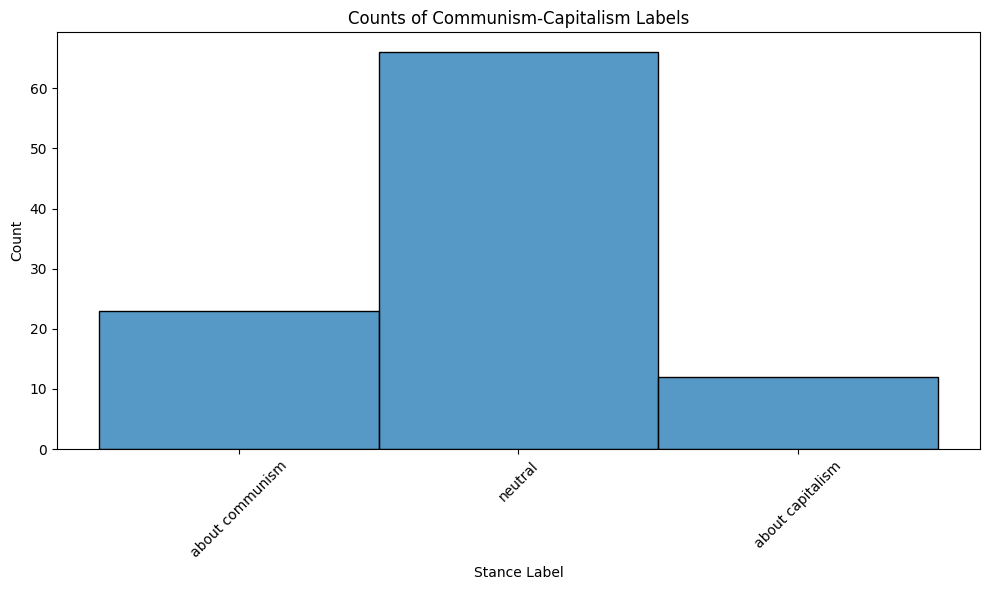
\includegraphics[width=0.45\textwidth]{plots/cap_comm_hist.png}}
    \subfigure{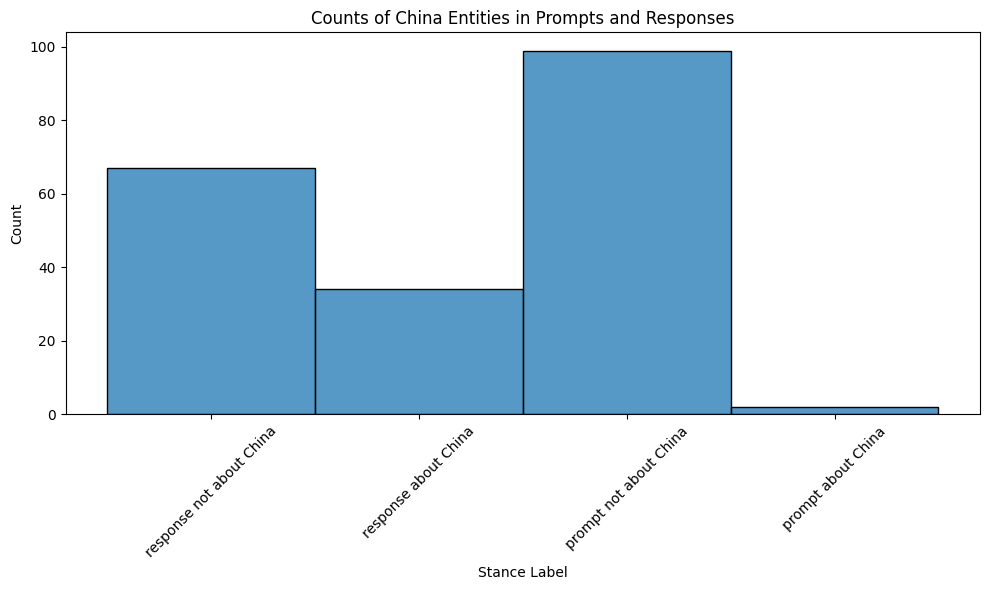
\includegraphics[width=0.45\textwidth]{plots/china_ent_hist.png}}
    \subfigure{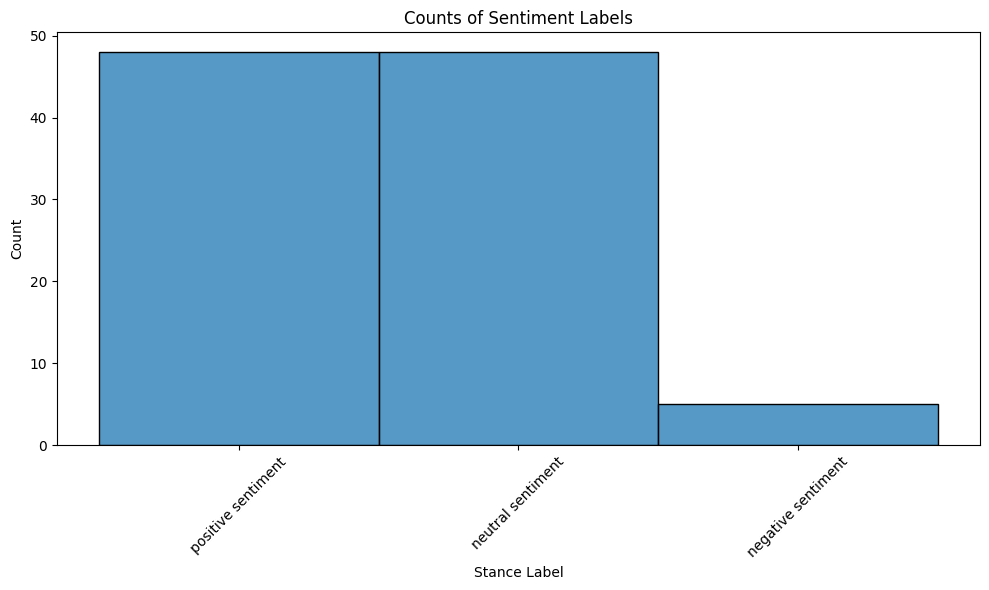
\includegraphics[width=0.45\textwidth]{plots/sentiment_hist.png}}
    \subfigure{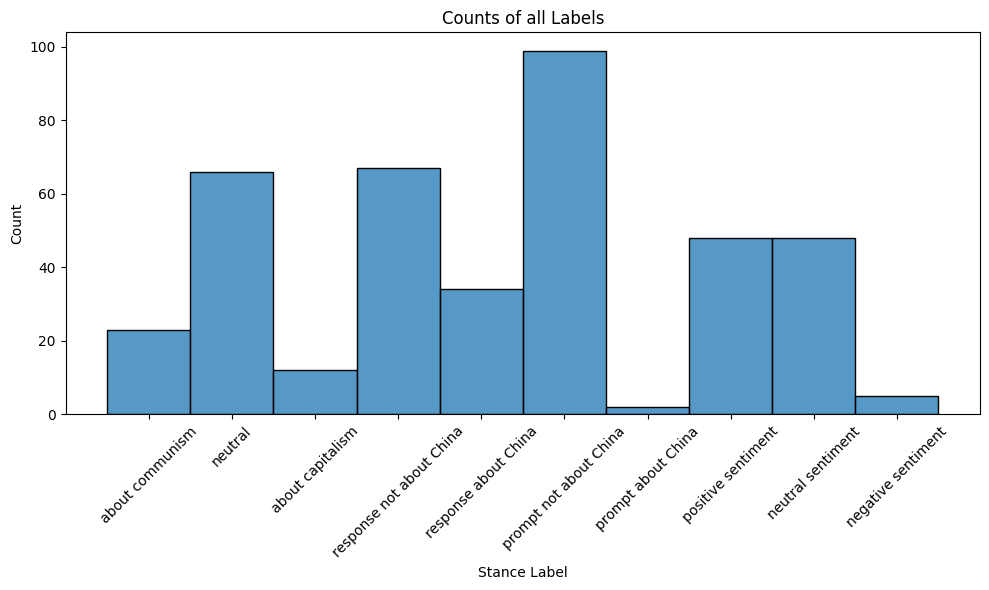
\includegraphics[width=0.45\textwidth]{plots/summary_hist.png}}
    \caption{counts of the occurences of labels}
    \label{fig:grid1}
\end{figure}

Comparing responses from political versus neutral prompts reveals that ideological biases are more pronounced when discussing governmental and economic systems. For instance, prompts such as "What are the drawbacks of communism?" and "Should more countries adopt capitalist policies?" tend to elicit responses with discernible stance preferences, while neutral questions such as "What are the benefits of spending time in nature?" yield less polarizing content.


\subsection{Analysis of Political and Sentiment Bias in Responses Related to China}
An interest finding consists in the fact that a considerable portion of the responses mention the government of China or his ruling party. To better understand the meaning and significance of this phenomenon a further analysis was required.

\begin{figure}[H]
    \centering
    \subfigure{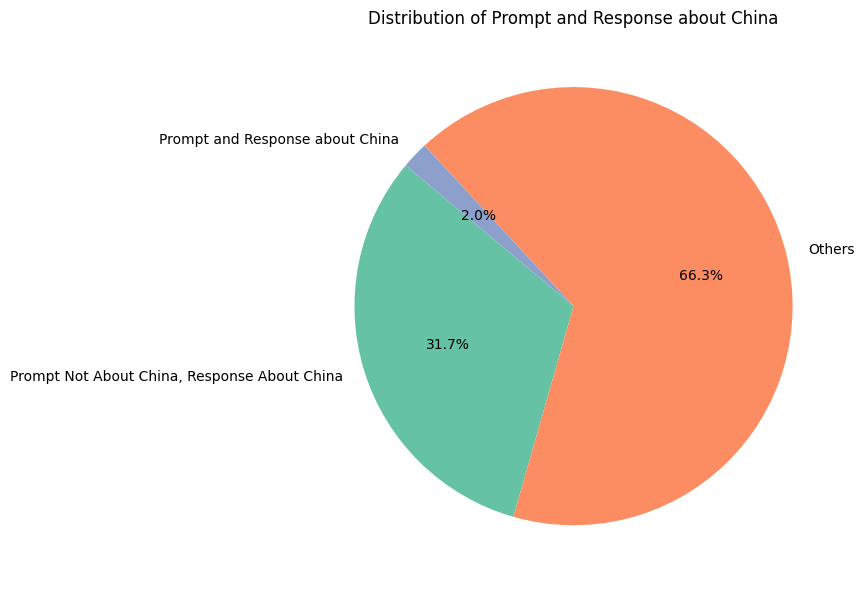
\includegraphics[width=0.45\textwidth]{plots/china_pie.png}}
    \subfigure{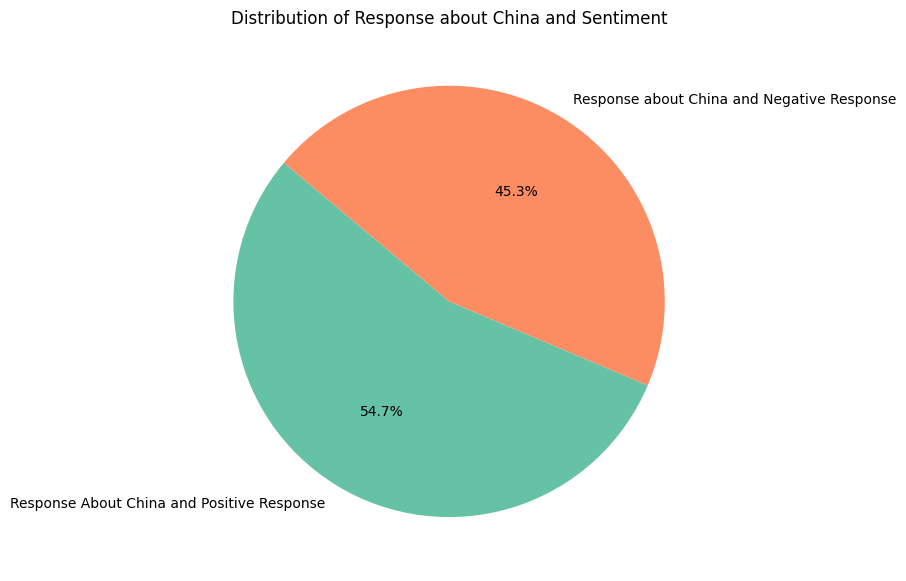
\includegraphics[width=0.45\textwidth]{plots/china_sentiment_pie.png}}
    \subfigure{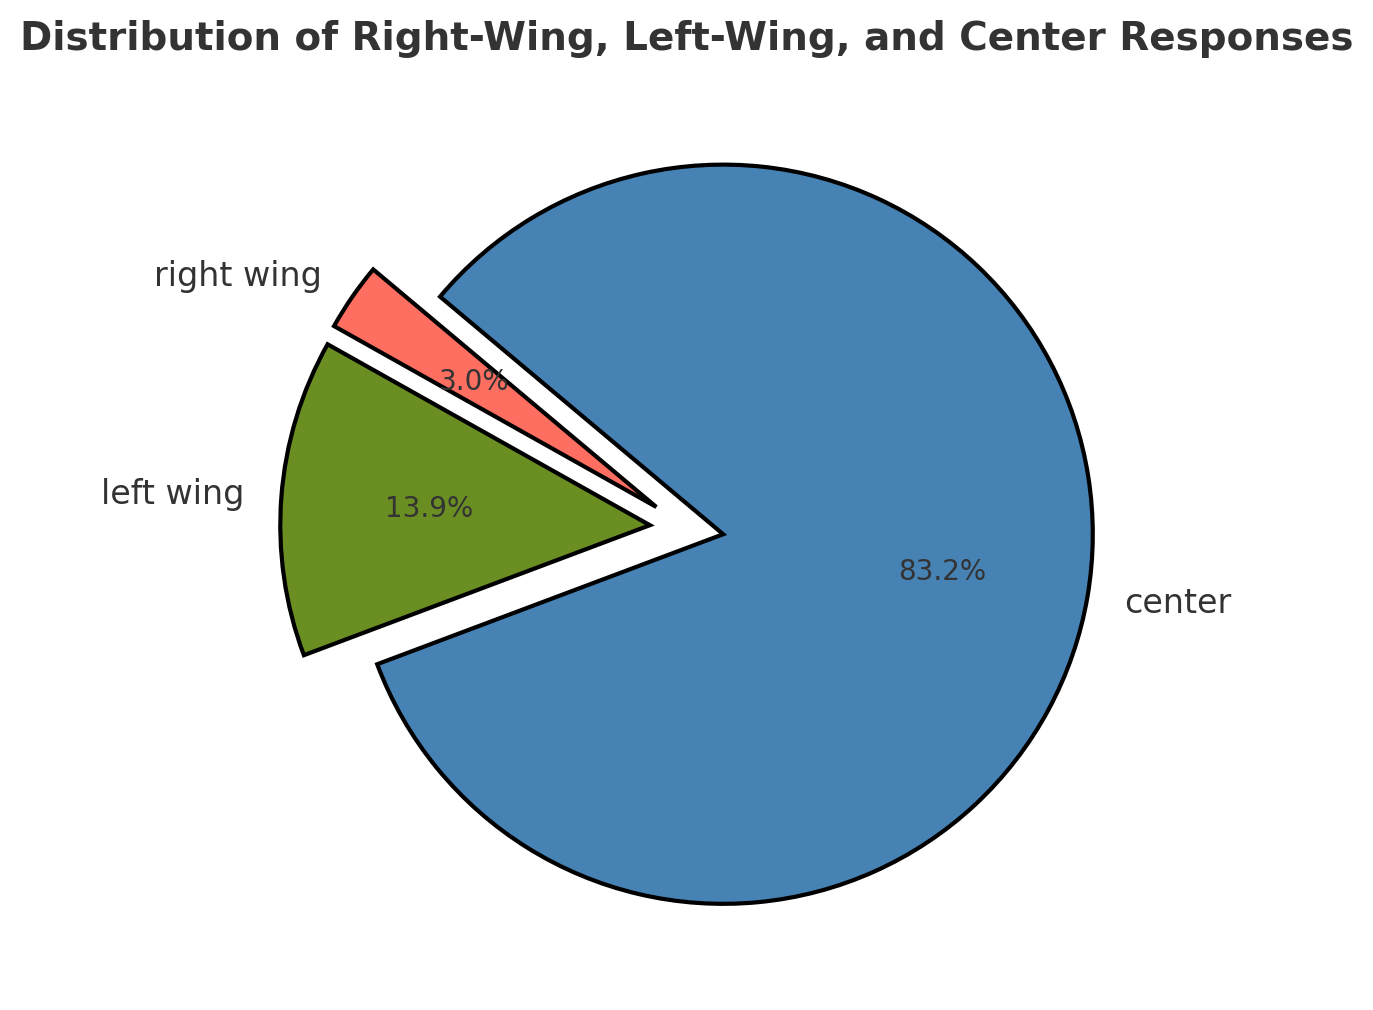
\includegraphics[width=0.45\textwidth]{plots/global_political_stand_pie.png}}
    \subfigure{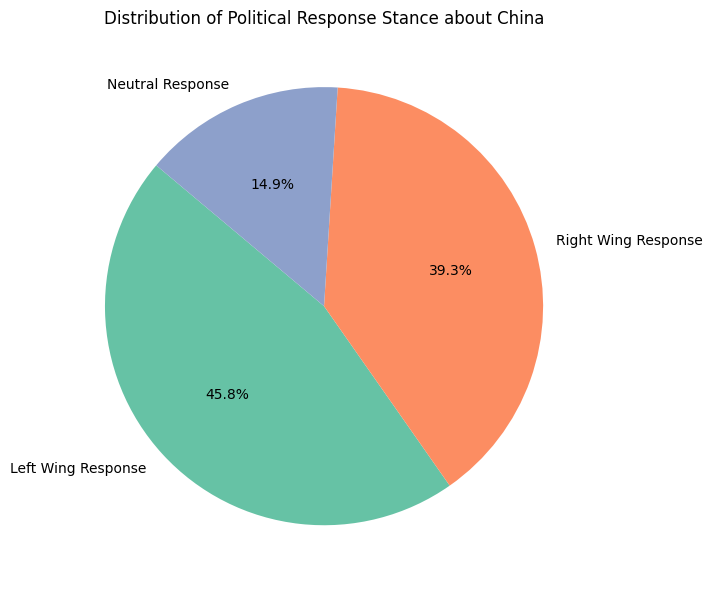
\includegraphics[width=0.45\textwidth]{plots/china_political_stand_pie.png}}
    \caption{distribution skews of labels occurency in China related responses}
    \label{fig:grid2}
\end{figure}

The first pie chart illustrates the frequency with which prompts and responses involve discussions about China. Notably, only 2.0\% of the interactions explicitly mention China in both prompt and response, while a significant 31.7\% of the responses bring up China despite the prompt not referring to it.
\\\\
The last pie chart categorizes responses regarding China into left-wing, right-wing, and neutral positions. The data suggests a slight lean toward left-wing responses (45.8\%), followed closely by right-wing responses (39.3\%), while neutral responses make up 14.9\%. The relatively high proportion of left-wing and right-wing stances indicates that responses about China tend to be politically charged rather than purely neutral.
\\\\
A broader view of political stance across all responses (not just those about China) is displayed in the third pie chart. Interestingly, 83.2\% of responses are neutral, while left-wing responses account for 13.9\% and right-wing responses for only 3.0\%. This stark contrast with the China-specific data suggests that discussions about China are significantly more polarized than other topics.

\subsection{Correlation Analysis of Political and Sentiment Biases}

To further assess the presence of political bias in text generation, we analyzed the correlations between various prompt and response labels, including political stance and sentiment. The correlation matrix (Fig. 3) highlights significant patterns in how the model generates responses across different political topics.

\begin{figure}[H]
    \centering
    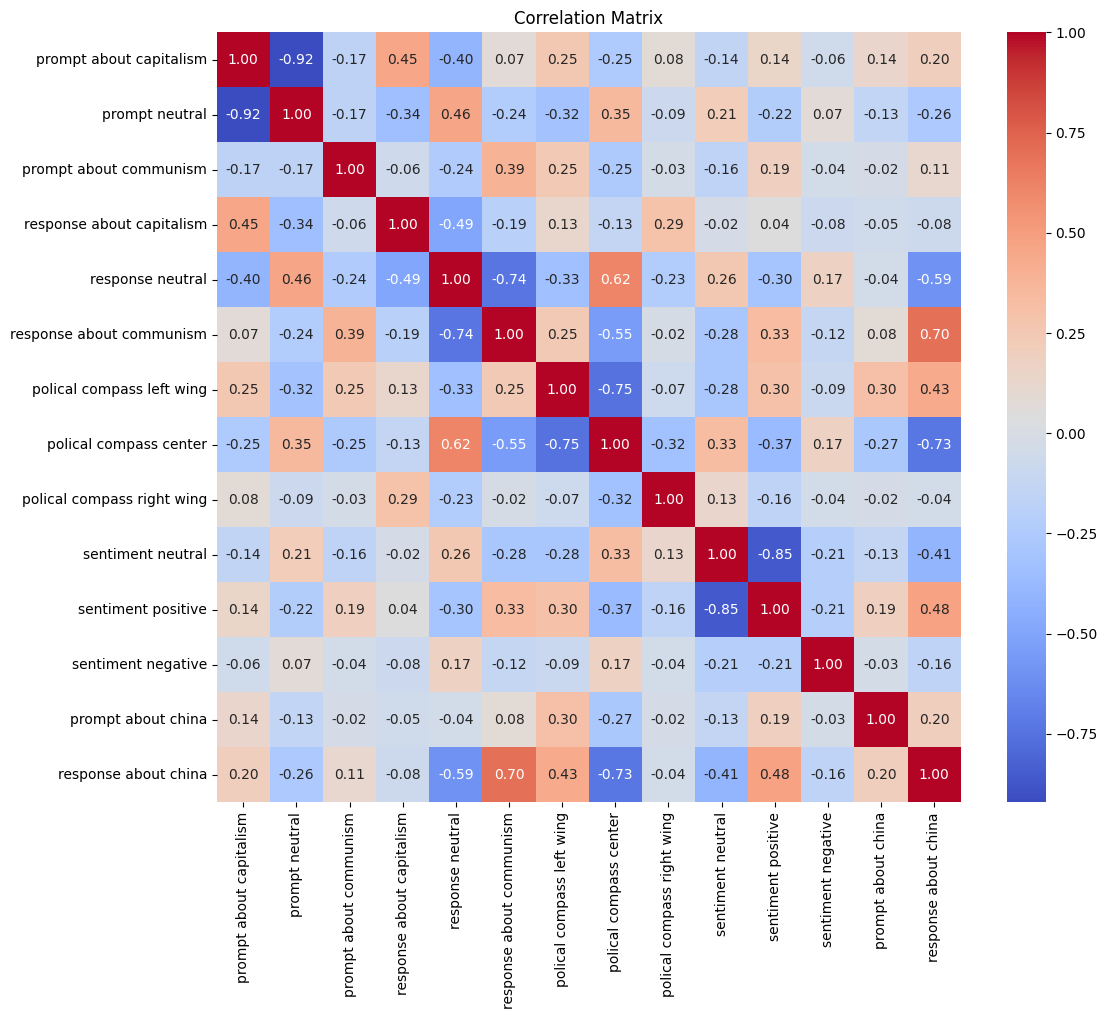
\includegraphics[width=\textwidth]{plots/corr_matrix.png} % Sostituire con il percorso dell'immagine
    \caption{correlatin matrix of all possible labels}
    \label{fig:3}
\end{figure}

\subsubsection{Topic Polarization and Non-Neutrality}

One of the most notable findings is the strong negative correlation between prompts about capitalism and neutral prompts (-0.92). This indicates that discussions on capitalism tend to be opinionated, rather than neutral. Similarly, responses discussing communism exhibit a strong negative correlation with neutrality (-0.74), suggesting that communism-related topics elicit stronger political stances.
\\\\
Interestingly, responses about China exhibit a moderately strong negative correlation with neutrality (-0.59), indicating that responses tend to take a stance rather than remain neutral.

\subsubsection{Political Leanings in Responses}

The data indicates subtle tendencies toward political leanings in responses. Left-wing responses show a slight positive correlation with discussions of communism (0.25), while right-wing responses exhibit a weak correlation with prompts about capitalism (0.29). Although these correlations are not strong, the model’s responses might reflect ideological biases when discussing economic systems. Additionally, neutral sentiment is negatively correlated with both left-wing and right-wing perspectives, while centrist perspectives correlate positively with neutrality (0.62). This suggests that politically charged responses—whether left-leaning or right-leaning—are less likely to be neutral.
\\\\
Responses about China strongly correlate with left-wing political stance (0.70) and negatively correlate with centrism (-0.73), indicating that discussions on China tend to align with left-leaning narratives rather than centrist or balanced viewpoints.
\\\\
These findings suggest that while the model does not overwhelmingly favor one ideology, it tends to frame China-related discussions from a left-leaning perspective.

\subsubsection{Sentiment Bias and Political Stance}

Sentiment analysis offers further insights into how political bias may manifest in AI-generated responses. The data suggests that left-leaning responses tend to be slightly more positive in tone, as indicated by a modest correlation of 0.30. This could point to a subtle tendency for left-wing narratives to be framed in a more favorable light compared to other perspectives.

Similarly, discussions about China show a moderate correlation with positive sentiment (0.48), suggesting that responses related to China are more likely to adopt a positive framing.

\section{Conclusion}

The study highlights the presence of political bias in the response of DeepSeek-R1-Distill-Llama-8 model, particularly in discussions on economic ideologies and geopolitics.
\\\\
Bias becomes more pronounced in China-related discussions, showing heightened polarization, with the topic frequently emerging even when not explicitly prompted. Sentiment analysis further reveals that left-leaning responses tend to be more positive, while discussions on China are moderately correlated with positive sentiment.
\\\\
Bias in stance distribution, topic selection, and sentiment framing raises concerns about AI’s impact on political discourse. Future research should focus on improving bias detection though a better prompt selection and mitigating these biases through dataset balancing, reinforcement learning, and improved transparency.

\bibliography{./sn-bibliography}
%% if required, the content of .bbl file can be included here once bbl is generated
%%\input sn-article.bbl

\end{document}
